\chapter{Vertikale Evolution} % 13 Seiten
Dieses Kapitel betrachtet die vertikale Evolution der agilen Softwareentwicklung. Wie bereits erörtert, befinden sich Vorgehensweisen und Prozesse in einem stetigen Wandel. Agile Vorgehensweisen haben viele Probleme der Softwareentwicklung bereits gelöst, sind jedoch nur auf diesen Bereich beschränkt. DevOps hingegen umfasst einige weitere Ebenen, wodurch sich deutlich umfangreichere Möglichkeiten ergeben. Diese werden nachfolgend betrachtet.


\section{Abgrenzung zu Lean und Agile} % 1 Seite
Neben DevOps besteht noch eine Vielzahl an weiteren Prozessen und Vorgehensweisen, welche verwandt, aufbauend, oder vollkommen eigenständig sind. Zwei der am weitest verbreiteten sind agile Entwicklung und Lean. Beide werden oft im Zusammenhang mit DevOps genannt. Manchmal werden diese jedoch fälschlicherweise synonym verwendet. Daher erfolgt zuerst eine Abgrenzung zu diesen beiden Vorgehensweisen.

\subsection{Lean}
Die Lean Bewegung, begründet im Lean Manufacturing und im IT Bereich geprägt von Eric Ries und dessen Buch \glqq The Lean Startup\grqq, verfolgt die Idee, der Prozessoptimierung und Konzentration auf Kernideen. Hierbei wird versucht, den Prozess von der Idee, über Ausarbeitung und Testing, hin zum fertigen Feature möglichst schlank und ressourcenschonend zu halten. Dies ist besonders im Startup Umfeld sehr interessant, da dort finanzielle Mittle meist recht knapp bemessen sind und die Produkte noch nicht genau definiert sind. Mit Hilfe von Lean kann frühzeitig Kundenfeedback eingeholt werden, was die Entwicklung des Produkts und die Definition eines Zielmarkts deutlich vereinfacht.\\
Lean verfolgt den Ansatz, sich auf einige wenige Kernideen zu konzentrieren und nur Probleme zu lösen, die in Zusammenhang mit diesen stehen und deren Lösung sich lohnt. \parencite[Vgl.][S. 18 ff.]{ries:2011} \\
Da es sich bei Lean, manchmal auch Lean Management genannt, um Optimierung von Prozessen und Organisation handelt, findet sich diese Vorgehensweise auch außerhalb der IT wieder.

\subsection{Agile}
Agile Softwareentwicklung ist, wie bereits beschrieben, eine iterativ, inkrementelle Vorgehensweise. Hierbei werden lauffähige Prototypen und kurzen Zyklen erstellt und dem Kunde präsentiert. Dadurch besteht die Möglichkeit, Feedback des Kunden bereits frühzeitig einzuholen und darauf zu reagieren. \parencite[Vgl.][S. 62]{Schatten:2010aa} Bedingt durch das iterative Vorgehen kann viel flexibler auf Änderungen der Spezifikation eingegangen werden und die Cost Of Change bleiben gering. Der Fokus liegt dabei auf Kollaboration mit dem Kunden und Bestreben, möglichst früh tatsächlichen Wert für den Kunden zu erzeugen. Agile Vorgehensmodelle umfassen allerdings keine weiteren Bereiche wie beispielsweise Betrieb, oder Management, sondern sind nur auf die Entwicklung von Software beschränkt.

\subsection{DevOps}
DevOps baut auf die beiden oben genannten Vorgehensmodelle Lean und Agile auf, geht aber über deren jeweiligen Umfang hinaus. So beinhaltet DevOps beispielsweise das Lean Prinzip der Optimierung der Durchlaufzeiten, oder das Agile Prinzip der möglichst frühen Generierung von Wert für den Kunden. DevOps konzentriert sich aber nicht nur auf die technischen Aspekte, sondern auch auf die organisatorischen und kulturellen Ebenen. Hierbei stehen Kollaboration von Entwicklung und Betrieb und kultureller Wandel im Vordergrund.\\
Es muss jedoch beachtet werden, dass eine optimal funktionierende Lösung oftmals aus der Anwendung einer Kombination und nicht nur aus einem der drei Modelle besteht.

\newpage
\section{Anwendung von DevOps in der Praxis} % 3 Seiten
Da es sich bei DevOps um ein Vorgehensmodell und nicht um ein fertig verfügbares Produkt handelt, kann die Anwendung in der Praxis, je nach Bedarf, viele unterschiedliche Formen annehmen. Nachfolgend werden beispielhaft die meist verbreiteten Möglichkeiten der Umsetzung dieser Praktiken vorgestellt.

\subsection{Organisatorisch}
Auf organisatorischer Ebene liegt der Fokus auf der Zusammenfassung der Abteilungen Entwicklung, Qualitätssicherung und Betrieb. Einer der Kernideen von DevOps ist die optimierte Kollaboration und Kommunikation in diesem Bereich. Um Wissen in einer Organisation möglichst transparent zu vorliegen zu haben, muss dieses durch Kommunikation und Kollaboration geteilt werden. Getrennte Abteilungen stellen hierbei jedoch meist sogenannte Silos dar, innerhalb derer Wissen unter Umständen geteilt wird, dieses aber normalerweise nicht nach Außen, beziehungsweise in andere Abteilungen gelangt. Durch die Anwendung von DevOps werden diese Silos abgeschafft und durch kollaborierende Teams mit geteiltem Wissen ersetzt. \parencite[Vgl.][S. 8]{huettermann:2012}
Eine Folge daraus ist, dass es keine Spezialisten klassischen Sinne mehr gibt. Teammitglieder müssen Fähigkeiten auf allen drei Gebieten, Entwicklung, Qualitätssicherung und Betrieb besitzen. Sie können aber immer noch bestimmte Kompetenzschwerpunkte besitzen. \parencite[Vgl.][S. 7]{sacks:2012}

\subsection{Technisch}
DevOps ist lediglich ein Vorgehensmodell, oder eine Sammlung von Praktiken, in dessen Umfeld sich allerdings diverse Tools zur Unterstützung entwickelt haben. Einige dieser Tools stammen ursprünglich aus verwandten Bewegungen, oder wurden von anderen Bewegungen übernommen. Die Popularität einiger dieser Tools außerhalb von DevOps trägt sicherlich auch zur Verbreitung von DevOps bei.\\

\begin{figure}[ht]
  \centering
  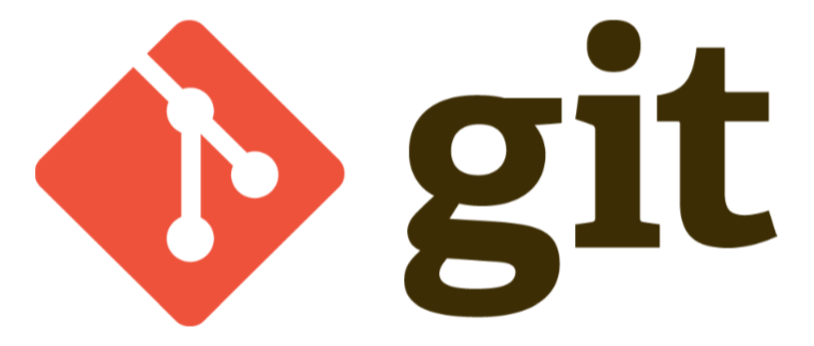
\includegraphics[width=0.2\textwidth]{img/git_logo.png}
  \caption{Git Versionsverwaltung \parencite[][]{Git:2016}}
  \label{fig:scrummodell}
\end{figure}

Bei DevOps werden alle in der Produktion entstandenen Artefakte an einer zentralen Stelle verwaltet. Dies geschieht in den meisten Fällen mit einer sogenannten Versionsverwaltung. Der Vorteil solcher Tools liegt darin, dass kollaborativ und ortstransparent an Artefakten gearbeitet werden und jegliche Änderungen genau dokumentiert werden. Somit befindet sich ein damit verwaltetes System immer in einem genau definierten Zustand. Es besteht auch die Möglichkeit, Änderungen ohne großen Aufwand rückgängig zu machen, oder unterschiedliche Versionen parallel zu verwalten.\\
Ein sehr bekannter Vertreter dieser Gattung von Tools ist Git. Es wurde entwickelt von Linus Torvalds, dem Erfinder von Linux, und hat sich mittlerweile zu einem sehr weit verbreiteten Versionsverwaltungstool entwickelt. Eines der Kernfeature ist die dezentrale Speicherung von Entwicklerrepositories, die es ermöglichen ortstransparent und effizient im Team zu kollaborieren. \parencite[Vgl.][S. 31 ff.]{loeliger:2012}

\begin{figure}[ht]
  \centering
  
\includegraphics[width=0.2\textwidth]{img/jenkins_logo.png}
  \caption{Jenkins Automatisierung \parencite[][]{Jenkins:2016}}
  \label{fig:scrummodell}
\end{figure}

Basierend auf dem Lean Prinzip der Optimierung, wird bei DevOps nicht nur die Organisation und Kollaboration optimiert, sondern auch auf technischer Ebene Entwicklung und Auslieferung. Als zentrales Element kommt hierbei oftmals eine Pipeline, in Form eines Continuous Integration Servers zum Einsatz. Eines der bekanntesten Open Source Projekte ist Jenkins. Dieses Projekt entstand aus dem Continuous Integration Server Projekt Hudson, nachdem dieses von Oracle aufgekauft wurde und viele Entwickler mit dessen Weiterentwicklung nicht mehr einverstanden waren. \parencite[Vgl.][S. 4]{smart:2011}\\
Ein Continuous Integration Server führt frei definierbare Aufgaben automatisiert aus und kann dabei mit unterschiedlichen Tools zusammenarbeiten. So kann er beispielsweise auf Änderungen in einer Versionsverwaltung reagieren und einen Bau- und Auslieferungsvorgang starten. Dabei können automatisierte Tests ausgeführt werden und das fertige Produkt auf verschiedene Systeme ausgeliefert werden. Die Einrichtung und Konfiguration solcher Continuous Delivery Server nimmt zu Beginn eines Projekts einige Zeit in Anspruch. Die zeitliche Ersparnis durch die vielen Möglichkeiten der Automatisierung gleichen diesen Aufwand aber wieder um ein Vielfaches aus. \parencite[Vgl.][S. 65 ff.]{smart:2011}\\
Continuous Integration Server bilden die Kerntechnologie bei DevOps, um eine schnelle Time To Market, schnelles Recovery nach Fehlerfällen, hohe Produktqualität und kurze Entwicklungszyklen zu erreichen.

\begin{figure}[ht]
  \centering
  
\includegraphics[width=0.2\textwidth]{img/chef_logo.png}
  \caption{Chef Konfigurationsverwaltung \parencite[][]{Chef:2016}}
  \label{fig:scrummodell}
\end{figure}

\begin{figure}[ht]
  \centering
  
\includegraphics[width=0.25\textwidth]{img/puppet_logo.png}
  \caption{Puppet Konfigurationsverwaltung \parencite[][]{Puppet:2016}}
  \label{fig:scrummodell}
\end{figure}

Ein weiteres Tool, welches Teil der Automatisierung ist und sehr gut mit einem Continuous Integration Server zusammen arbeitet ist eine Konfigurationsverwaltung. Diese Tools ermöglichen es, Konfigurationen zentral zu verwalten und automatisiert ablaufen zu lassen. Bei der manuellen Konfiguration von Servern und Systemen kommt es oft vor, dass sich Systeme in unterschiedlichen Zuständen befinden auf Grund unterschiedlicher Versionen, oder unterschiedlichen Herangehensweisen bei der Einrichtung. Dies bedeutet nicht nur bei der initialen Konfiguration, sondern auch bei allen darauf folgenden Updates und Upgrades einen erhöhten Zeitaufwand. Nicht standardisierte Systeme bedeuten auch im Fehlerfall einen erhöhten Aufwand bei der Suche und Beseitigung. Mit Hilfe von Konfigurationsverwaltungen erfolgt die Konfiguration aller System automatisiert, identisch und wiederholbar. Somit sinkt der Aufwand bei der initialen Konfiguration, bei Updates und Upgrades und im Falle eines Fehlers deutlich. Bekannteste Vertreter sind die Tools Chef und Puppet. Beide bieten eine sehr ähnlichen Grundfunktionalität, sind aber spezialisiert auf unterschiedliche Einsatzgebiete. \parencite[Vgl.][S. 1 ff.]{krum:2014} \parencite[Vgl.][S. 8 ff.]{taylor:2014}

\begin{figure}[ht]
  \centering
  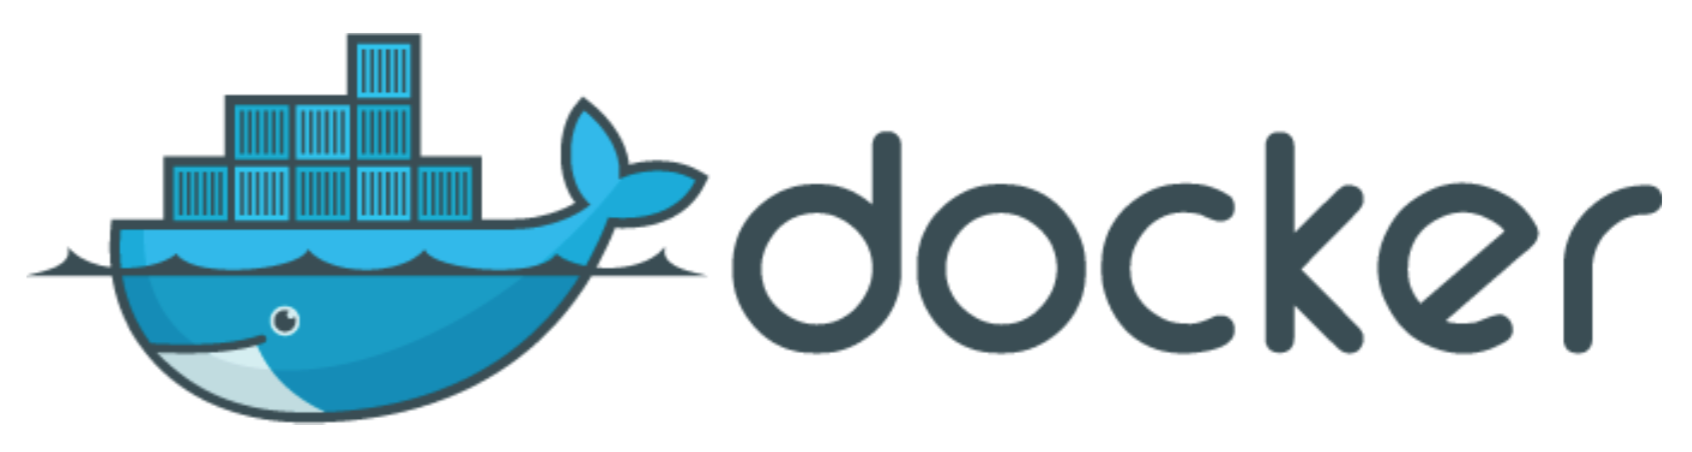
\includegraphics[width=0.4\textwidth]{img/docker_logo.png}
  \caption{Docker Deployment \parencite[][]{Docker:2016}}
  \label{fig:scrummodell}
\end{figure}

Das Deployment, oder Auslieferung, bildet das abschließende Element einer automatisierten Pipeline. Hier werden alle Produktionsartefakte zu einem lauffähigen System zusammengefasst und auf die entsprechende Infrastruktur ausgeliefert. Beispielsweise die Installation einer Shop Applikation auf einem Webserver. In diesem Bereich gab es in den letzten Jahren auf Grund steigender Performanz bei Hardware und Software große Sprünge in der Entwicklung. Dies führt dazu, dass Infrastruktur, beziehungsweise Plattformen virtualisiert werden können. Damit vereinfacht sich die Entwicklung und die Auslieferung um ein Vielfaches. Ein solches Tool zur Auslieferung und Virtualisierung ist Docker.\\
Docker ermöglicht es, ein System vollkommen identisch beliebig oft auszuliefern. Somit kann es bei der Auslieferung von Systemen keine Probleme mehr in Form von unterschiedlichen Konfigurationen, oder Installationen geben. Auch die Entwicklung profitiert von Virtualisierung, da so Betriebsumgebungen im Kleinformat zur Entwicklung genutzt werden können und es keine Unterschiede mehr zwischen Entwicklung und Betrieb gibt. Zudem erhöht Virtualisierung die Sicherheit, da einzelne Systeme vollständig getrennt auf dem selben Server arbeiten können und Angreifer nicht zwischen diesen wechseln können. \parencite[Vgl.][S. 3 ff.]{matthias:2015}

\subsection{Kulturell}
Ein oft vergessener, aber durchaus wichtiger Teil von DevOps ist der kulturelle Aspekt. Um diesen genauer betrachten zu können müssen zuerst die unterschiedlichen Kulturformen einer Organisation erörtert werden.
Nach Westrum \parencite[Vgl.][]{westrum:2004} gibt es drei unterschiedliche Arten von Organisationen:

\begin{itemize}
\item Machtorientierte Organisationen
\item Bürokratische Organisationen
\item Generative und Leistungsorientierte Organisationen
\end{itemize}

In machtorientierte Organisationen gibt es nur sehr wenig Kooperation und Kollaboration. Zudem wird Scheitern als sehr negativ angesehen und meist nicht akzeptiert. Mitarbeiter arbeiten nur für den eigenen Vorteil und versuchen sich selbst möglichst unentbehrlich darzustellen. In einer solchen Art der Organisation gibt es nur sehr geringe, oder gar keine Innovation, da Mitarbeiter nicht gewillt sind, Risiken einzugehen und neue Richtungen einzuschlagen.\\
Bürokratische Organisationen zeichnen sich dadurch aus, dass jede Abteilung und jeder Mitarbeiter genau definierte Aufgaben und Ziele haben. Von diesen wird nicht abgewichen, auch wenn sich dadurch ein Vorteil für einen Einzelnen, oder das Team entstehen würde. In dieser Art der Organisation herrscht oftmals Angst vor Veränderungen und Neuerungen, dementsprechend findet auch hier nur sehr geringen, oder aber gar keine Innovation statt. Kollaboration und Kooperation werden nur angewendet, wenn dies genau vorgegeben ist.\\
In generativen und leistungsorientierten Organisationen findet hingegen sehr viel Kooperation und Kollaboration statt. Es herrscht ein fehlerverzeihendes Umfeld, in dem Mitarbeiter dazu ermutigt werden, Risiken einzugehen und eventuell zu scheitern, da alle Mitarbeiter dadurch lernen können. Mitarbeiter arbeiten an einem gemeinsamen Ziel und teilen die dabei entstehenden Risiken, anstatt sie einzelnen Abteilungen, oder Personen zuzuschreiben. In einer solchen Organisation existiert keine Art der \glqq über die Mauer werfen\grqq Mentalität, bei der Probleme \glqq über die Mauer\grqq an andere Abteilungen weitergegeben werden, ohne diese zu lösen, um eigenen Ressourcen zu schonen. Jeder Mitarbeiter hat eine Verantwortung für die Qualität, die Verfügbarkeit und die Sicherheit des Produkts. Ein solches Umfeld fördert Innovation und das Beschreiten neuer Wege.\\
DevOps strebt eine generative und leistungsorientierte Organisationskultur an, bei der Mitarbeiter, besonders die der Abteilungen Entwicklung, Qualitätssicherung und Betrieb in hohem Maße kollaborieren und kommunizieren. Durch die Zusammenfügung verschiedener Abteilungen wird das Risiko auf alle Mitarbeiter gleichermaßen verteilt und alle sind für die Qualität des Produkts verantwortlich. Nur so lässt sich ein innovatives und effizientes Umfeld aufbauen, weshalb die kulturelle Ebene für DevOps von so großer Wichtigkeit ist.

\newpage
\section{DevOps im Projektmanagement und ITIL} % 2 Seiten
Nachdem im vorangegangenen Abschnitt auf die praktische Umsetzung von DevOps eingegangen wurde, wird nun betrachtet, welche Anpassungen in Organisationen vorgenommen werden müssen, in denen andere Vorgehensmodelle eingesetzt werden und DevOps zum Einsatz kommen soll.

\subsection{Projektmanagement}
Um DevOps in einer Organisation einzusetzen, müssen entsprechende Anpassungen im Projektmanagement vorgenommen werden. Da DevOps keine Praktiken für Projektmanagement beinhaltet, kann hier auf bereits bestehende Vorgehensmodelle aufgebaut werden. Die umfangreichste Anpassung ist die Aufhebung der Trennung der Abteilungen der Entwicklung, der Qualitätssicherung und des Betriebs. Hierbei müssen die bestehenden Silos aufgelöst werden und ein gemeinsames Management für das gesamte Team geschaffen werden.\\
Bei der Projektplanung muss beim Einsatz von DevOps berücksichtigt werden, dass keine getrennten Phasen für Qualitätssicherung und Testen notwendig sind, sondern stattdessen Zeit für die Erstellung und Einbindung automatisierter Tests in die Entwicklungsphase eingeplant werden muss.\\
Durch den Einsatz von DevOps besteht zudem die Option, Fortschritt nicht nur in Textform als Bericht, sondern in Form lauffähiger Prototypen zu demonstrieren. Dies ist eine der wichtigsten Eigenschaften agiler Vorgehensmodelle, bei denen zum Sprint Ende, im Durchschnitt alle zwei Wochen, ein solcher Prototyp an den Kunde ausgeliefert wird. Mit Hilfe von DevOps ist es möglich, Prototypen mehrmals am Tag zu erzeugen. Mittels der automatisierten Pipeline entsteht aus jeder Änderung ein solcher Prototyp.\\
Ein weiterer Vorteil, den der Einsatz von DevOps mit sich bringt, ist das \glqq Design for Failure\grqq. In klassischen Projekten muss eine Fehlerstrategie extra erarbeitet werden. Bei DevOps besteht diese zum einen aus Standardisierung und Protokollierung jeglicher Änderungen, wodurch Fehlersuche sehr stark vereinfacht. Zum anderen besteht diese Strategie aus einem sehr schnellen Recovery, bedingt durch den hohen Grad an Automatisierung. Im Falle eines Fehlers, oder eines Ausfalls kann ein neues System automatisiert in kürzester Zeit neu ausgeliefert werden. Dies ist besonders bei cloudbasierten Diensten, oder Webapplikationen wie Online Shops von besonderer Bedeutung, da hier Ausfallzeiten besonders hohe finanzielle Auswirkungen haben. \parencite[Vgl.][]{Null:2014}

\subsection{ITIL}
ITIL ist im Bereich des IT Managements ein internationaler \glqq De-facto-Standard\grqq und findet daher in vielen IT Abteilungen Anwendung. Um DevOps in solch einem Umfeld einsetzen zu können, müssen keine vollkommen neuen Strukturen geschaffen werden, sondern DevOps kann parallel zu ITIL eingesetzt werden. Dies ist ein großer Vorteil von DevOps, da die Veränderung vorhandener Strukturen mit Kosten verbunden ist. So kann DevOps zunächst in geeigneten Bereichen getestet werden und bei Bedarf ausgebaut werden.\\
Zur Einführung von DevOps in ITIL orientierte Bereiche wurde folgende Vorgehensweise entwickelt:

\begin{itemize}
\item Identifizierung der ITIL Prozesse
\item Review der Prozesse
\item Identifizierung der Schwachstellen
\item Konkrete Planung
\item Priorisierung und Umsetzung
\end{itemize}

\parencite[Vgl.][]{Sharp-Paul:2016}

Zunächst werden geeignete Bereiche im entsprechenden Umfeld identifiziert, in denen ein ausreichend großer Vorteil durch Automatisierung und verbesserte Zusammenarbeit entstehen kann. Daraufhin werden die wichtigsten ITIL Prozesse in diesen Bereichen identifiziert. Nach diesem Schritt werden die ausgewählten ITIL Prozesse einem Review unterzogen. Dieser findet mit allen an diesen Prozessen beteiligten Abteilungen statt. Nur so kann sichergestellt werden, dass der Einsatz von DevOps an dieser Stelle optimal und ohne Verlust ist. Um den Aufwand und die Dauer hierbei in Grenzen zu halten, können diese Reviews als Workshop veranstaltet werden. Auf das Review folgt nun die Identifizierung der Schwachstellen der jeweiligen ITIL Prozesse. Hierbei liegt der Fokus darauf, welche Fehler den höchsten Schaden verursachen können. Dabei werden die Eintrittswahrscheinlichkeit und die Kosten im Falle eines Fehlers untersucht. Anschließend werden konkrete Maßnahmen definiert, wie in diesen Prozessen Automatisierung und Kollaboration gewinnbringend eingesetzt werden können. Dies geschieht nun auf einem niedrigeren Abstraktionsniveau und liefert als Ergebnis die tatsächlich geplante Umsetzung. In einem letzten Schritt folgt eine Priorisierung der einzelnen ITIL Prozesse und Maßnahmen und die tatsächliche Umsetzung. \parencite[Vgl.][]{Sharp-Paul:2016}

\newpage
\section{Optimierungspotentiale und Verbreitung} % 1 Seiten
In diesem Abschnitt werden die Optimierungspotentiale von DevOps im Vergleich zu bereits bestehenden Vorgehensmodellen und die Verbreitung von DevOps aufgezeigt. Hierzu wurde der \glqq State Of DevOps Report 2015\grqq \parencite[Vgl.][]{DevOpsSODR:2015} und ein Report von Gartner \parencite[Vgl.][]{Gartner:2015} ausgewertet. In diesem Report wurden IT-Führungskräfte befragt, auf welche Art und Weise DevOps eingesetzt wird und welche Vorteile sich durch diesen Einsatz ergeben haben.

\begin{figure}[ht]
  \centering
  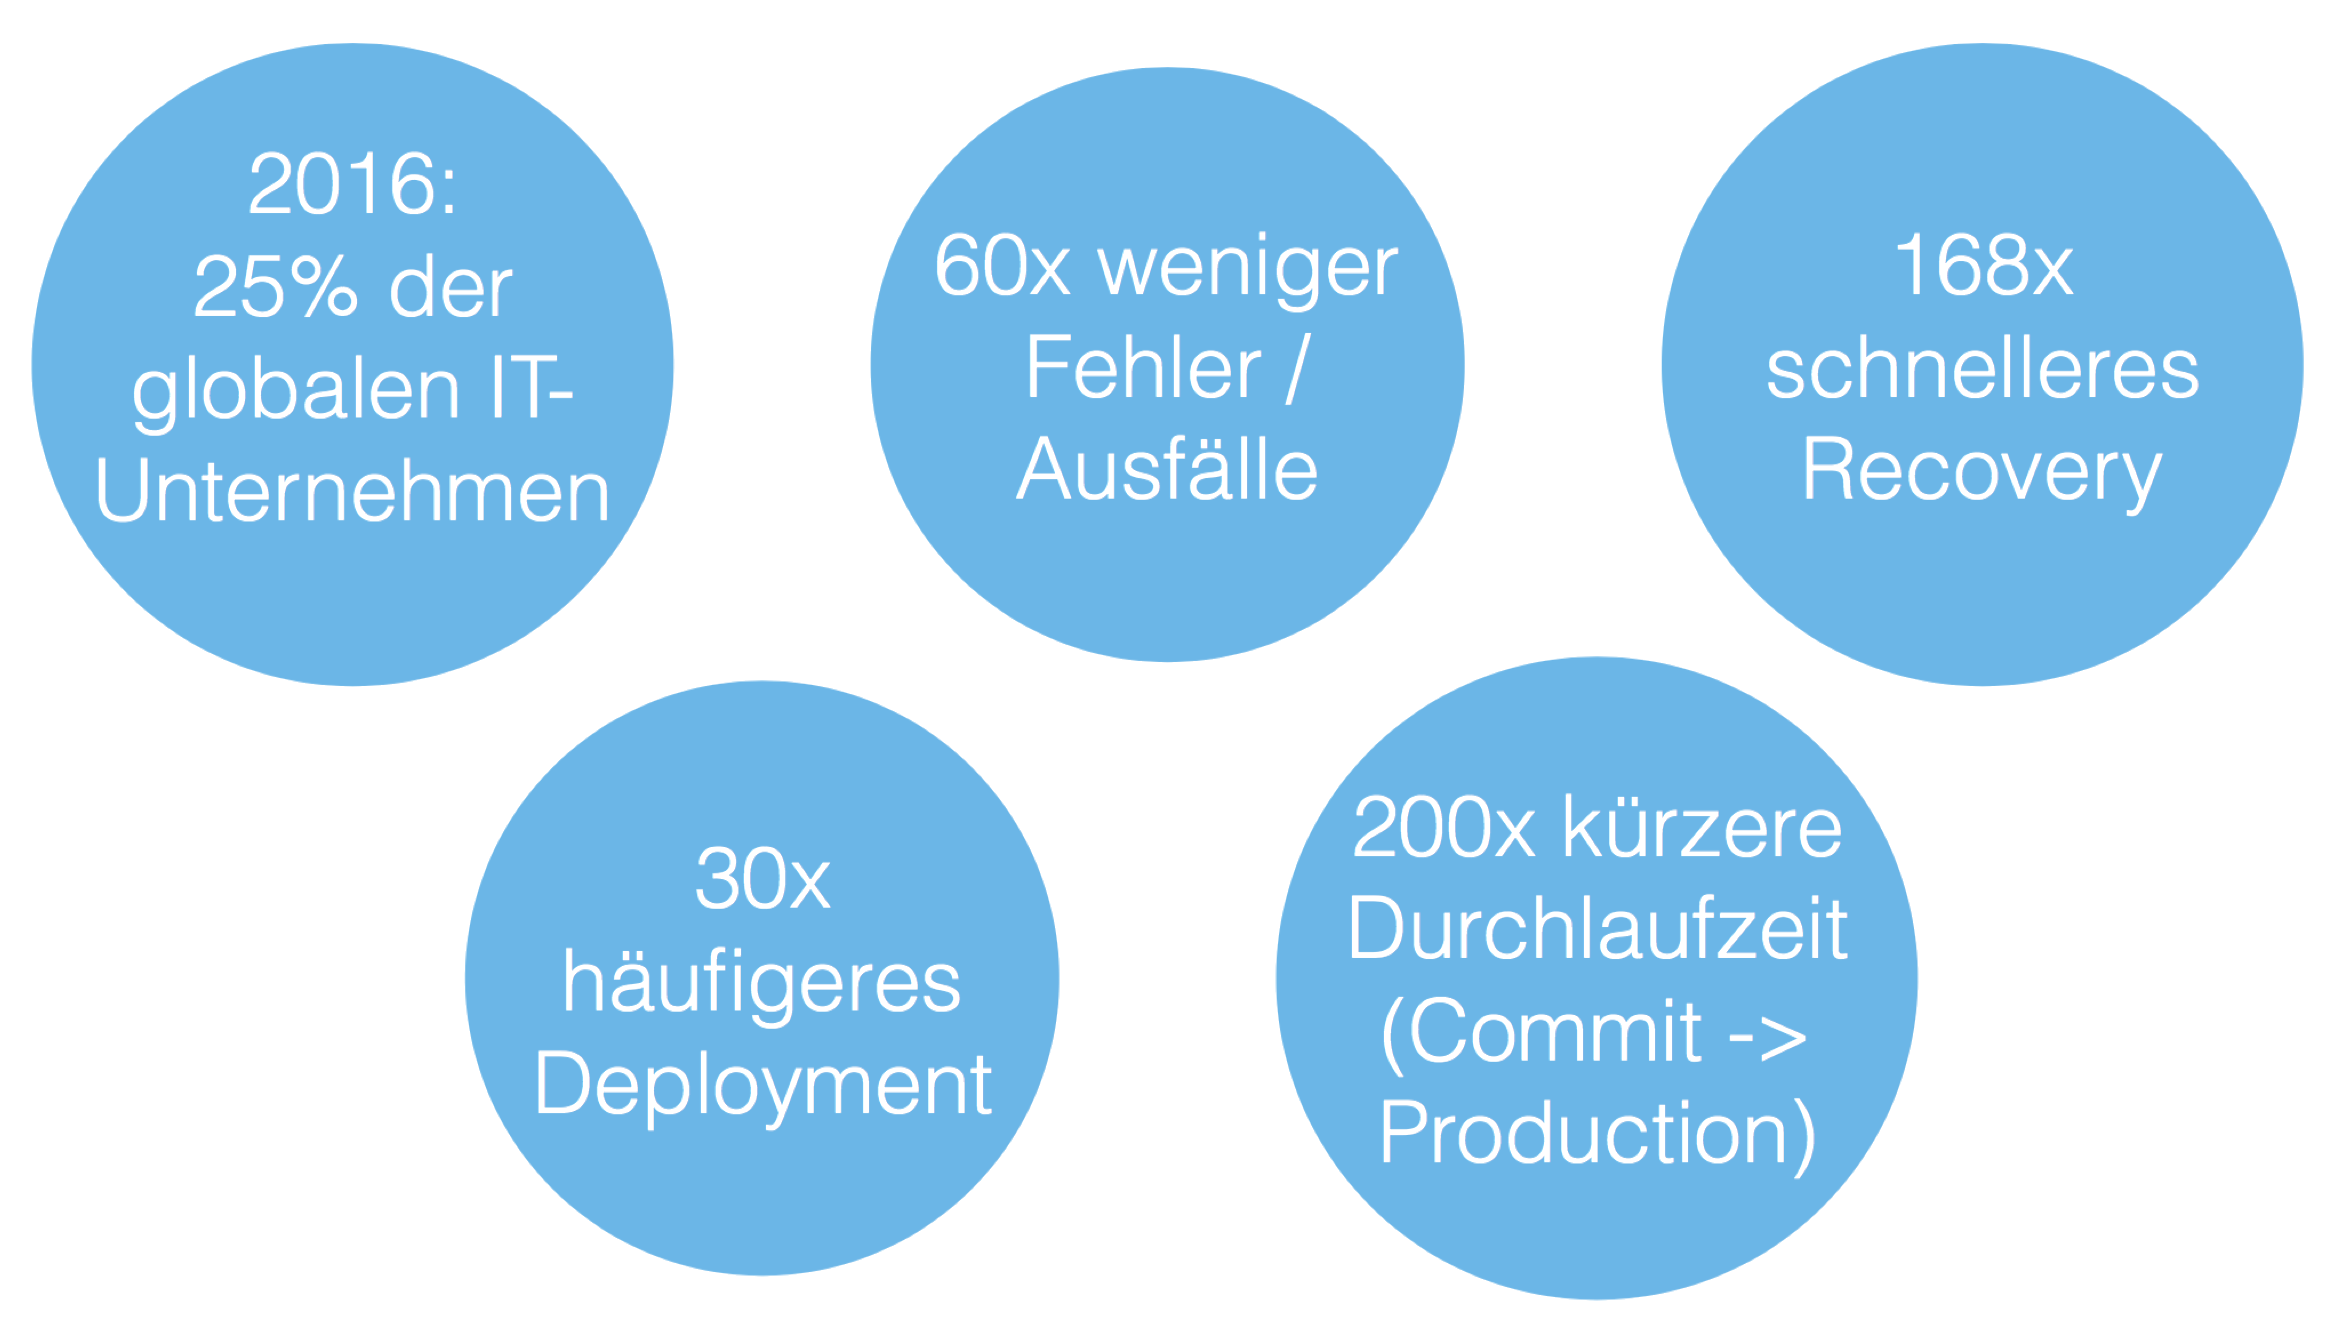
\includegraphics[width=\textwidth]{img/devops_zahlen.png}
  \caption{Verbreitung und Potentiale von DevOps}
  \label{fig:scrummodell}
\end{figure}

\subsection{Optimierungspotentiale}
Die Optimierungspotentiale von DevOps kommen größtenteils durch den hohen Grad an Automatisierung, standardisierte und automatisierte Konfigurationsverwaltung, automatisiertes Deployment und kulturellen Wandel in Form von besserer Kollaboration und Kommunikation zustande. Hierbei lassen sich 30 fach häufigeres Deployment und eine 200 fach kürzere Durchlaufzeit feststellen. Änderungen, die von Entwicklern am System vorgenommen werden, durchlaufen Qualitätssicherung und Auslieferung um ein Vielfaches schneller, da große Teile dieses Prozesses automatisiert sind. Auch die Qualität des Produkts wird durch den kulturellen Wandel und automatisierte Tests mit Hilfe von DevOps deutlich erhöht, was zu 60 fach weniger Ausfällen führt im Vergleich zu vorher bestehenden Entwicklungs- und Auslieferungsprozessen. Ein weiterer Nebeneffekt der Automatisierung ist ein 168 fach schnelleres Recovery im Falle eines Fehlers. Die automatische Wiederherstellung eines Systems ist um ein Vielfaches schneller als eine manuelle Wiederherstellung. Dies führt zu kürzeren Ausfallzeiten und deutlich geringeren finanziellen Schäden. \parencite[Vgl.][]{DevOpsSODR:2015}

\subsection{Verbreitung}
DevOps war in den Anfangsjahren eher eine Nischen Bewegung, die hauptsächlich in Cloud und Mobile Bereichen zum Einsatz kam. In den Jahren 2014 und 2015 hat das Wachstum der Verbreitung stark zugenommen \parencite[Vgl.][]{DevOpsSODR:2014}, \parencite[Vgl.][]{DevOpsSODR:2015}. Dem Gartner Report \parencite[Vgl.][]{Gartner:2015} zufolge wird das Wachstum von DevOps im Verlauf des Jahres 2016 weiter stark zunehmen und zu einer Verbreitung von 25 Prozent weltweit führen.

\newpage
\section{Aktuelle Entwicklung von DevOps} % 3 Seiten
Die DevOps Bewegung ist eine selbst für Informatik Verhältnisse noch junge Bewegung, deren Entwicklung in stetigem Wandel ist und noch lange nicht abgeschlossen ist. Aktuelle Entwicklungen beschäftigen sich mit der Integration von Sicherheit in den Prozess. Diese Entwicklung ist für diesen Bericht auch daher von Interesse, da hier einer der Unterschiede zu den bereits etablierteren agilen Vorgehensmodellen gesehen werden kann. Insbesondere zu den weiterentwickelten Modellen, die im Kapitel \glqq Horizontale Evolution\grqq betrachtet werden und die Sicherheit als eines ihrer Kernelement bereits enthalten.

\subsection{DevOps und Sicherheit}
Bisherige praktische Umsetzungen der DevOps Praktiken, insbesondere auf technischer Ebene in Form von automatisierte Pipelines, beinhalteten keine sicherheitsrelevanten Elemente. Sicherheit wurde, wie in der klassischen Entwicklung, als ein auf die Entwicklung folgender \glqq Flaschenhals\grqq betrachtet. Da die Geschwindigkeit in klassischen, oder auch agilen Vorgehensmodellen, deutlich unter der Geschwindigkeit von DevOps lag, fiel dies bisher nicht so stark ins Gewicht. Mit stark verkürzten Durchlaufzeiten und einer immer kürzeren Time To Market wird die fehlende Integration von Sicherheit in die DevOps Prozesse zu einem immer größeren Problem, das die Entwicklung stark ausbremst. Allerdings bietet DevOps einige sehr gute Eigenschaften, welche den Aufbau einer performanten Sicherheitsstrategie sehr gut unterstützen. Hierzu müssen beim Einsatz von DevOps bereits vorhandene Sicherheitsstrategien angepasst werden.

\subsection{Automatisierte Sicherheit}
Ein Element von DevOps, welches zu einer performanten Sicherheitsstrategie beiträgt, ist automatisierte Auslieferung. Somit ist sichergestellt, dass alle sicherheitsrelevanten Konfigurationen auf allen Systemen immer exakt identisch sind. Zudem können Sicherheitstests in die Pipeline integriert werden, wodurch alle Änderungen, die am System vorgenommen werden, automatisch überprüft werden.\\
Systeme, die in Organisationen entwickelt werden, die DevOps Praktiken einsetzen, werden automatisiert konfiguriert und installiert. An bereits installierten Systemen werden keine manuellen Änderungen durchgeführt. Wenn es in der Entwicklung zu einer Änderung kommt, wird diese durch die automatisierte Pipeline verarbeitet, getestet und auf die entsprechenden Systemen ausgeliefert. Es gibt bei der Verwendung von DevOps keine Updates mehr, sondern nur noch Upgrades. Diese Art von Upgrade ist auch als \glqq Phoenix Upgrade\grqq bekannt. Dabei wird das System bei jedem Upgrade vollständig neu ausgeliefert und installiert. Dieses Vorgehen zieht keinen zusätzlichen Aufwand nach sich, da all diese Vorgängen automatisiert ausgeführt werden.Für die Sicherheit des Systems bedeutet solch ein Vorgehen jedoch einen großen Vorteil gegenüber bisherigen Systemen. So können jegliche Artefakte des Systems über entsprechende Rechtevergabe als unveränderlich konfiguriert werden. Sollte ein Angreifer Zugriff auf ein solches System erlangen, kann er keine Manipulationen an diesem durchführen.\\
Bei DevOps wird auch, wie bereits erwähnt, die Konfiguration als Teil des Systems gesehen. Diese wird mittels Virtualisierung in Form von Software entwickelt und verwaltet. Auf diese Art und Weise können Konfigurationsartefakte, genauso wie Systemartefakte, mit unveränderlichen Rechten auf dem Endsystem ausgestattet werden. Da diese ebenso nur per Upgrade, jedoch niemals per Update verändert werden, greift auch dort diese Art der Sicherung vor Manipulation. Diese Art der Konfiguration wird auch als \glqq Immutable Infrastructure\grqq, oder \glqq Wegwerf Infrastruktur\grqq \parencite[Vgl.][S. 16]{matthias:2015} bezeichnet.\\
Ein weiterer Aspekt von DevOps, der weniger der direkten Bedrohung durch Angreifer entgegenwirkt, sondern viel mehr die Verfügbarkeit von Systemen betrifft, ist die automatisierte Auslieferung. Wie bereits im Abschnitt der \glqq Optimierungspotentiale\grqq erwähnt, lässt sich mit deren Hilfe die Time To Recover deutlich reduzieren. Es besteht jedoch auch die Möglichkeit, Upgrades des Systems möglichst sicher auszuliefern, sodass die Ausfallzeiten Idealfall bei Null liegen. Dies ist besonders relevant für die E-Commerce Branche. Diese besondere Art des Upgrades ist bekannt unter dem Namen \glqq Blue-Green Upgrade\grqq, oder \glqq Blue-Green Deployment\grqq. \parencite[Vgl.][S. 103 f.]{bass:2015} Dabei wird ein Upgrade zunächst nur auf ein Teil des Systems ausgeliefert. Das System ist zu diesem Zeitpunkt in alter Version immer noch erreichbar. Falls das Upgrade ohne Probleme funktioniert hat und entsprechende Systemtests bestanden wurden, kann auf das neue System umgestellt werden und der alte Teil des Systems ebenfalls per Upgrade aktualisiert werden. Sollte der Upgrade fehlschlagen kann die alte Version, da diese in der Versionsverwaltung vorliegt, schnell wiederhergestellt werden. Durch dieses Vorgehen ist das System jederzeit erreichbar und Upgrades können performant und sicher durchgeführt werden.\\
Grundsätzlich besteht auch ohne DevOps die Möglichkeit, ein solches Upgrade durchzuführen. Allerdings ist dies bei manueller Durchführung deutlich langsamer und kostenintensiver, da das Upgrade jedes Elements des Systems manuell durchgeführt werden muss. Zudem müssen für die Übergangsphase, in der Teile des Systems eine alte und Teile des Systems eine Version besitzen, oftmals extra Systeme angemietet werden. Diese Kosten sind bei automatisierten Auslieferung deutlich geringer. Ein Rollback auf einer ältere Version ist manuell nur schwer möglich, da im Normalfall nicht genau dokumentiert ist, ob und welche manuellen Änderungen, oder Updates am System vorgenommen wurden. Somit kann es unter Umständen unmöglich sein, eine alte Version wieder exakt herzustellen.\\

\subsection{Auditierung und Compliance}
Auditierung und Compliance können mitunter sehr kosten- und zeitintensiv sein. Auch hierbei kann der Einsatz von DevOps Zeit und damit Kosten sparen, da Auditierung und Compliance vereinfacht werden können. Da alle Artefakte zentral in einer Versionsverwaltung gespeichert und verwaltet werden, werden alle Änderungen genau protokolliert. Zudem befindet sich das System jederzeit in einem genau definierten Zustand, der über die Artefakte bestimmt werden kann. In bisherigen Modellen und Prozessen sind nicht alle Artefakte zentral verwaltet, wodurch nicht alle Änderungen protokolliert werden und der Zustand des Systems aufwendig bestimmt werden muss. Auditierungen mit Hilfe von DevOps deutlich optimierter durchgeführt werden. Die automatisierte Pipeline von DevOps bietet zudem die Möglichkeit, nicht nur automatisierte Sicherheitstests zu integrieren, sondern auch automatisierte Compliance Tests zu integrieren. Dadurch kann sichergestellt werden, dass alle Änderungen, die am System vorgenommen werden, mit den Compliance Vorgaben übereinstimmen.\\

\subsection{Security as Software}
Wie bereits erwähnt liegt dieser Bereich von DevOps aktuell im Fokus der Entwicklung. Die Vision, auf die hingearbeitet wird, ist \glqq Security as Software\grqq. Ziel dieser Vision ist die vollständige Integration der Sicherheit eines Systems in die automatisierte Pipeline. Da diese softwarebasiert ist, müssen alle Elemente des Sicherheitssystems in Form von Software vorliegen. Da Automatisierung immer einen gewissen Grad an Abstraktion fordert, ist dieses Vorhaben entsprechend komplex. Erste Schritte sind mit \glqq Infrastructure as Software\grqq, der damit verbundenen \glqq Immutable Infrastructure\grqq, \glqq Phoenix Upgrades\grqq und ersten automatisierten Sicherheitstests als Teil der Pipeline bereits getan. Sollte hier ein Durchbruch und damit die vollständige Integration der Sicherheit in die Pipeline gelingen, so würde dies die Vorteile von DevOps und dessen Attraktivität noch deutlich erhöhen und dessen Anwendbarkeit deutlich erweitern.

\newpage
\section{Fallstudie} % 3 Seiten
Die folgende Fallstudie zeigt beispielhaft die Einführung und Einbettung von DevOps in bereits vorhandene Vorgehensmodelle und Prozesse in einer Organisation. Sie zeigt die Einführung von DevOps bei Nordstrom, einem Fashion Retailer aus Nordamerika, der Boutiquen, Einkaufszentren und einen Online Shop betreibt.

\begin{figure}[ht]
  \centering
  
\includegraphics[width=0.5\textwidth]{img/nordstrom_logo.png}
  \caption{Nordstrom Logo \parencite[][]{Nordstrom:2016}}
  \label{fig:scrummodell}
\end{figure}

\subsection{Einführung}
Nordstrom hatte vor der partiellen Einführung von DevOps ein klassische Aufteilung der Abteilungen. So gab es in der IT unter anderem getrennte Abteilungen für Entwicklung, Qualitätssicherung und Betrieb. \parencite[Vgl.][S. 1]{Reed:2014} Bedingt durch die Trennung der Abteilungen waren die Update Zyklen für die Homepage, den Online Shop und die Kassensysteme in den Boutiquen sehr lang. Updates der Systeme wurden manuell durchgeführt, meist über Nacht, um den dabei anfallenden Schaden durch Ausfallzeiten möglichst gering zu halten. Trotzdem dauerte ein Update der Homepage eine komplette Nacht. Besonders manuelle Änderungen, die nicht korrekt dokumentiert wurden und im Nachhinein ausgeführt wurden, waren ein sehr großes Problem. Diese mussten nach dem Upgrade identisch durchgeführt werden, was oftmals zu großen Verzögerungen geführt hat. Ein weiteres Problem waren die Unterschiede zwischen Entwicklungs- und Produktionsumgebungen. Die Entwickler entwickelten die Systeme auf ihren eigenen Entwicklungsumgebungen, die sich aber zum Teil stark von den Produktionsumgebungen unterschieden. Die Systeme konnten zwar im Anschluss an die Entwicklung entsprechend getestet werden, aber Probleme, die in Zusammenhang mit der Produktionsumgebung auftraten, konnten dabei allerdings nicht getestet werden und führten beim Update Vorgang zu großen Verzögerungen.\\
Bedingt durch die vielen manuell durchgeführten Schritte bei der Konfiguration und Installation der Systeme konnte nur langsam auf Probleme reagiert werden. Auf Grund mangelhafter Dokumentation, nicht reproduzierbarer Schritte und unterschiedlichen Konfigurationen in den Umgebungen war die Suche nach Fehlern stark erschwert und hat im Falle eines Ausfalls großen finanziellen Schaden nach sich gezogen. \parencite[Vgl.][S. 3]{Reed:2014}

\subsection{Optimierungspotentiale durch DevOps}
Der thematisch interessanteste und kundenwirksamste Bereich DevOps zu testen wäre die Homepage gewesen. Allerdings ist dieser Bereich auch mit einem sehr hohen Risiko verbunden, daher wurde für die Einführung von DevOps der Bereich der Bezahlsysteme in den Boutiquen ausgewählt. Hierbei sind Umfang und Risiko überschaubar und die Abhängigkeiten zu anderen Bereichen relativ gering.\\
Die Bezahlsysteme in den einzelnen Boutiquen bestehen aus den Kassen und einem Server, der die Transaktionen lokal verwaltet und mit dem Hauptsystem in Verbindung steht. Die lokalen Server waren vor der Einführung von DevOps Windows 2003 Server, die manuell vor Ort konfiguriert und installiert wurden. Updates mussten ebenso manuell vor Ort durchgeführt werden. Diese wurden von Technikern in zwei Schichten innerhalb von 18 Stunden pro Server durchgeführt. Auch hier gab es die bereits erwähnten Probleme mit fehlender Dokumentation manuell durchgeführter Änderungen und Probleme auf Grund unterschiedlicher Konfigurationen der Entwicklungs- und Produktionsumgebungen. \parencite[Vgl.][S. 5]{Reed:2014}\\ 
Durch die Einführung von DevOps sollte zum einen auf organisatorischer und kultureller Ebene die Kollaboration und Kommunikation zwischen Entwicklung, Qualitätssicherung und Betrieb deutlich verbessert werden. Dadurch sollte die Anzahl von Fehlern, die auf Grund unterschiedlich konfigurierter Umgebungen der einzelnen Abteilungen entstanden sind, minimiert werden. Auch sollten Probleme, die bei der Auslieferung auftreten könnten und von der Entwicklungsabteilung vorhergesehen werden könnten, besser kommuniziert werden, um die Auslieferung möglichst reibungslos zu gestalten. Ein weiteres Ziel war es, die Verantwortung für das Produkt zu teilen, auf ein gemeinsames Ziel hin zu arbeiten und somit die Qualität des Produkts zu steigern. Auf technischer Ebene sollten die Server in den Boutiquen virtualisiert werden und der Entwicklungs- und Auslieferungsprozess bestmöglich automatisiert werden. Das Ziel der Virtualisierung der Server ist, dass es keine Unterschiede mehr zwischen den Entwicklungs- und Produktionsumgebungen mehr gibt. Somit können Entwickler auf kleinen Versionen der Produktionsumgebungen entwickeln, sodass es bei der Auslieferung keine unvorhergesehenen Probleme mehr auftreten. Durch die Automatisierung des Entwicklungs- und Auslieferungsprozesses sollte die Durchlaufzeit von Änderungen deutlich verringert werden. Mit Hilfe von automatisierten Tests sollte die Qualität der Änderungen und des kompletten Produkts erhöht werden und mit einer automatisierten Auslieferung sollte die manuelle und zeitintensive Auslieferung vor Ort abgelöst werden. Ein Nebeneffekt der Automatisierung der Auslieferung ist eine sehr schnelle Reaktionszeit auf Fehler und Ausfälle. Im Falle eines Fehlers kann somit die aktuelle Version in kurzer Zeit erneut ausgeliefert werden um den Fehler zu beheben. Ein weiterer Vorteil ist die erhöhte Sicherheit gegen Manipulation der lokalen Server, durch \glqq Immutable Infrastructure\grqq. \parencite[Vgl.][S. 5]{Reed:2014}\\

\subsection{Durchführung und Ergebnis}
Nachdem Optimierungspotentiale durch eine Einführung von DevOps identifiziert wurden, wurde deren konkrete Ausführung und Auswirkung in einem Team bestehend aus Entwicklern der Server und Datenbank, Mitarbeitern der Qualitätssicherung und Ingenieuren, die die manuelle Auslieferung bisher durchgeführt hatten, auf technischer Ebene erarbeitet.\\
Diese Mitarbeiter bildeten während der anschließenden Durchführung das DevOps Team. Das Team hatte ein gemeinsames Management und alle Teammitglieder arbeiteten in den Bereichen Entwicklung, Qualitätssicherung und Betrieb, jeweils mit eigenen Kompetenzschwerpunkten. \parencite[Vgl.][S. 4]{Reed:2014}\\
Nach mehreren Wochen Arbeit entstand ein vollautomatisiertes System. Alle Artefakte werden nun zentral verwaltet, Änderungen durchlaufen automatisierte Tests, um die Qualität sicherzustellen und die Auslieferung erfolgt vollkommen automatisch. Dadurch verringert sich der zeitliche Aufwand von 18 Stunden Auslieferung pro lokalem Server auf 4 Stunden vollautomatisierter Erstellung und Auslieferung auf allen bestehenden Systemen, ohne manuelle Arbeit vor Ort. Durch diesen Grad an Automatisierung sind alle Schritte beliebig Wiederholbar und können im Falle eines Fehlers erneut ausgeführt werden. Somit kann auch sehr schnell auf Fehler, oder Ausfälle im Betrieb reagiert werden. Die Qualität der Systeme konnte durch die Virtualisierung zudem deutlich gesteigert werden, da die Entwicklungsumgebungen exakt den Produktionsumgebungen gleichen und somit alle Eigenschaften, besonders das Verhalten unter hoher Last, schon während der Entwicklung getestet werden können. \parencite[Vgl.][S. 6]{Reed:2014}\\
Da das Ergebnis dieses Versuchs so erfolgreich war, wurde bei Nordstrom beschlossen die Einführung von DevOps weiter voran zu treiben. \parencite[Vgl.][S. 14]{Reed:2014}
